Per stimare la percentuale di problemi individuati da tre valutatori è stato fatto riferimento alla \textit{curva di Nielsen} (Figura \ref{curva_nielsen}), che modella la probabilità cumulativa di rilevazione dei problemi in funzione del numero di valutatori coinvolti. 

Assumendo che la probabilità che un singolo valutatore identifichi un problema sia pari a $L = 0.31$, la probabilità che almeno uno dei tre valutatori rilevi un determinato problema è:
\[
  1 - (1 - L)^3 = 1 - (1 - 0.31)^3 \approx 0.672
\]

ossia circa il 67.2\% dei problemi effettivamente presenti. Secondo il modello di Nielsen, ci si aspetta quindi che tre valutatori siano in grado di individuare complessivamente il 67.2\% dei problemi dell'interfaccia.

A partire da questa stima, si può ricavare il numero totale di problemi presenti. Indicando con $P$ il numero di problemi rilevati e con $N$ il numero totale di problemi esistenti, si ha:
\[
  P : N = 67.2 : 100
\]

\noindent
Poiché i tre valutatori hanno identificato $P = 93$ problemi unici, si ottiene:
\[
  93 : N = 67.2 : 100
\]

\noindent
Da cui segue:
\[
  N = \frac{93 \times 100}{67.2} \approx 138
\]

\noindent
Pertanto, il \textit{numero totale di problemi stimati} nell'interfaccia risulta essere circa 138.

\begin{figure}[H]
  \centering
  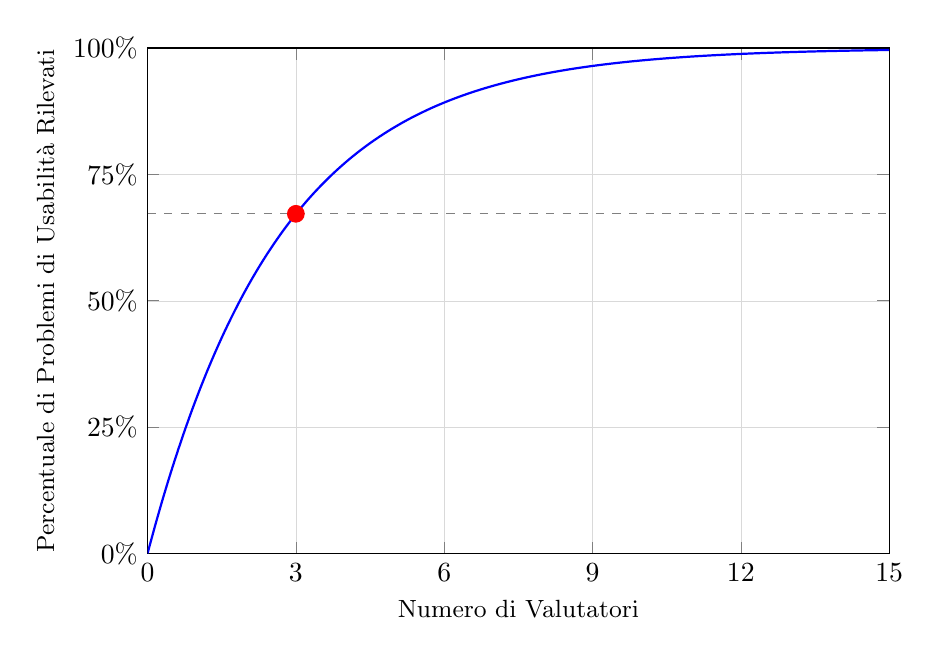
\begin{tikzpicture}
    \begin{axis}[
        width=11cm,
        height=8cm,
        xlabel={Numero di Valutatori},
        ylabel={Percentuale di Problemi di Usabilità Rilevati},
        xmin=0, xmax=15,
        ymin=0, ymax=100,
        xtick={0,3,6,9,12,15},
        ytick={0,25,50,75,100},
        yticklabels={0\%,25\%,50\%,75\%,100\%},
        grid=major,
        grid style={line width=.1pt, draw=gray!30},
        xlabel style={font=\small},
        ylabel style={font=\small, align=center},
      ]

      % Curva di Nielsen (L=0.31)
      \addplot[domain=0:15, samples=100, smooth, thick, blue]
      {100*(1 - (1-0.31)^x)};

      % Linea tratteggiata orizzontale al 67.2%
      \addplot[dashed, gray, thin] coordinates {(0,67.2) (15,67.2)};

      % Punto per 3 valutatori
      \addplot[mark=*, mark size=3pt, red, only marks]
      coordinates {(3, 67.2)};

    \end{axis}
  \end{tikzpicture}
  \caption{Curva di Nielsen.}
  \label{curva_nielsen}
\end{figure}